\chapter{Methods}
\label{chaptermethods}
In this chapter, I will explain the experimental methods I take in order to asses the performance of the Segmented feature set compared to the performance of the Full and SHARP feature set. For my first goal, I will begin by outlining how I will classify models, giving a precise definition for how one model ``performs better" than another and stating the statistical hypothesis test I wish to show. Then, I will explain some of the invalid hits in my highest performing model (the Artificial Neural Network), and why they may have occurred so I can fix the problem space and model in my second goal.

I will then describe the precise steps I took in order to optimize the model. Optimizing my highest performing model isn't only about optimizing hyper parameters, it also involves tuning the problem statement itself. I.e what is it I am actually trying to predict? Essentially, how can I phrase and design my model the best way that offers the most useful information to solar flare forecasters?

\section{Goal One: Segmentation vs No Segmentation / SHARPs}
My first goal in this study is to show that Segmentation is a novel feature extraction method that allows for an improvement over similar parameterization without segmentation. In order to show this goal, I will first show that the given a representative subset of machine learning models, Segmented data tends to perform better over it's control (Full). Then, I will dive deeper into the best performing (overall) model, and examine how it classifies flares by looking at how well it predicts positive outcomes and negative outcomes. I will also look at the ARs it fails on and by explaining why the model fails, I will better be able to optimize the model in my second goal. 

For the rest of this study, I will utilize a skill metric called the true skill statistic. It's meaning and derivation can be found in appendix \ref{appendix:judjingcriteria}. Generally, though, it measures the performance of a model with equal weights to positive rates and negatives rates within a feature set. See \ref{appendix:judjingcriteria} for a more detailed description.  

A model $M$ is said to perform better on a feature set $D_1 = D_{train1} \cup D_{test1}$ than $D_2 = D_{train2} \cup D_{test2}$ if, after training the model on a training subset $D_{test1} \subset D_1$ that is ``irrelevant" from a testing subset $D_{test1} \subset D_1$, the TSS score of model $M$ on $D_1$ ($TSS(M(D_{test1}))$) is greater than the TSS score on on $D_2$ ($TSS(M(D_{test2}))$):

$$TSS(M(D_{test1})) > TSS(M(D_{test2}))$$

A feature set $D_{test}$ is irrelevant from $D_{train}$ if it is:

\begin{enumerate}
    \item Disjoint from $D_{train}$:
    $$D_{train} \cap D_{test} = \emptyset$$
    \item Has none of the same HARP numbers in either set:
    $$\forall u \in D_{train} \quad (\nexists v \in D_{test} \quad HARP number(u) = HARP number(v))$$
\end{enumerate}

More conditions could be added to this irrelevancy operator, such as avoiding ARs within a certain distance or time of one another, but these two stated conditions are sufficient for the purposes of this study. These conditions ensure that we are not overfitting our data on arbitrarily placed training data. That is, we want our model to work for new data, not previously trained data. Normally, a validation feature set is also used to help with stopping conditions and optimizations, but for the purposes of this study, only a train and test feature set are considered.

Also, it is critical that the test feature set models the real world. We can do this by matching a few (2 in this study - the ratio of M and X flares) global metrics that are found in the field with the test feature set. Consider a set of ARs that do or do not produce an $M$ or $X$ class flare collected from the Helioseismic magnetic imager over time and the two associated ratios in this feature set:

\begin{itemize}
    \item $\frac{N_x^+}{N}$ - Number of ARs that produce an X class flare ($N_x^+$) over the number of ARs observed over in the feature set ($N$).
    \item $\frac{N_m^+ - N_{mx}^+}{N}$ - Number of ARs that produced only an M class flare ($N_m^+ - N_{mx}^+$) over the number of ARs observed in the feature set ($N$).
\end{itemize}

In the real world, these two ratios vary greatly with time. The roughly 11 year solar cycle shows that flares occur over a pattern of highs and lows. Also, there are other global ratios that are important such as the ratio of $C$, $B$, $A$ class flares or the ratio of flares that occur over one section of the sun compared to another section of the sun. Ideally, our test feature set would match all these ratios perfectly, however, in this study, I apply the principle of Randomized Block Design. That is, we have a few known variables (produces M or X class flare) with a known variation and a (theoretically infinite) number of unknown variables with unknown variance (location on the sun, time of year, etc) that we wish to match between our test feature set and the real world, however, we don't have this type of control, so we separate the data by the variables we do know and uniformly sample datapoints from these two blocks so that the other unknown variables are as uniformly distributed as possible. I have calculated the above two ratios and forceFully created the test feature set so that the data points match these ratios. 

From the period of 1996-11-24 17:31:00 to 2018-06-18 8:47:00, there have been a recorded 2015 flaring events of type $M$ and $X$ that range over the NOAA AR numbers 7999-12713. Because NOAA ARs are the input we look at in practice to forecast flares, we will rely on the ratios with respect to the NOAA AR classification convention rather than JSOC's HARP number naming system, although there is very little difference between the two. NOAA ARs are labeled if they are observed by two or more observatories, and are labeled consecutively, so we can estimate there have been a total of $4714 \quad (12713 - 7999)$ ARs that could have been classified in the field. Note that this time gap is approximately 22 years, which spans approximately 2 solar cycles. If we sampled slightly earlier or later, there could be more or fewer flares depending on the activity of the sun. This specific date range ensures we are sampling uniformly across solar cycles.

In this time period, there have been 575 NOAA ARs that produced an M flare ($N_x^+$), 78 NOAA ARs that produced an X flare ($N_m^+$), 75 NOAA ARs that produced both X and M flares ($N_{mx}^+$) (showing that most AR's that produce X flares also produce M flares!)

So we wish to match the ratios: $\frac{N_x^+}{N} = \frac{74}{4714} = 0.0157$ and $\frac{N_m^+ - N_{xm}^+}{N} = \frac{575 - 75}{4714} = 0.106$

In my feature set, there are 139 SHARPs ARs that produced an M flare, 21 SHARPs ARs that produced an X flare, 13 SHARPs ARs that produced both X and M flares and 739 total SHARPs ARs

To ensure our training to test split is approximately $0.7$, assume we remove $p\%$ of our class $X$ flaring HARP numbers and move them to our testing set. Then $N_{x}^+ = 21p$. Now, we also know $N_{mx}^+$ by counting the number of these chosen HARP numbers that also produce $M$ flares. We have two knowns ($N_x^+$, $N_{mx}^+$) and two unknowns ($N_m^+$, $N$). By solving the constraints outlined above (in terms of $p$, and $N_{mx}^+$ is non fixed / randomized):

$$N = \frac{1}{0.0157}N_x^+=\frac{21}{0.0157}p$$
$$N_{m}^+ = 0.106N + N_{mx}^+$$

I wish to make $\frac{N}{739} = 0.7 \rightarrow p = \frac{0.0157*0.7*739}{21} = 0.3867$

Therefore, to create a train / test split:

\begin{enumerate}
    \item I take $8$ random X flaring HARP numbers and move them to the test feature set (and all of their associated dates)
    \item Of the $8$ HARP numbers chosen, I count how many of them also produce an $M$ flare and calculate $N_{m}^+ = 0.106*517 + N_{mx}^+$ and take this many ARs from the set of $M$ HARP numbers and move them to the testing feature set.
    \item I fill the rest of the test feature set with non flaring HARP numbers to meet the number of required datapoints in the test set: $N$.
\end{enumerate}

After splitting the data into a train test split where the test data models the real world as best as possible, I train the given model $M$ on the training feature set and compute the $TSS$ (appendix \ref{appendix:judjingcriteria}) score of the test feature set. 

Of course, the results of a single model often vary, so repeating this train test process is crucial to maximize the benefits of the randomized block design. I repeat the above process for model $M$ 50 times and collect the TSS score for each trial. I now have two iid random variables which has taken the values: $TSS_{D1} = \{tss1_{d1}, tss2_{d1}... tss50_{d1}\}$ and $TSS_{D2} = \{tss1_{d2}, tss2_{d2}... tss50_{d2}\}$. I wish to show that $\bar{TSS}_{D2} \neq \bar{TSS}_{D1}$ with certainty. A two tailed statistical hypothesis can be formulated with the null hypothesis ($H_0$) and alternate hypothesis ($H_A$):

$$H_0: \mu = \bar{TSS}_{D1} - \bar{TSS}_{D2} = 0$$
$$H_A: \mu = \bar{TSS}_{D1} - \bar{TSS}_{D2} \neq 0$$

where $\bar{TSS}$ is the actual (not sample) mean of $TSS$. Using a $z-test$ because $n > 30$, I use the $\alpha = 0.01$ level threshold to confidently say that the $TSS$ score produced by feature set 1 ($D1$) is different than the $TSS$ score produced by feature set 2 ($D2$), and I simply order the two by rank. If $TSS_{D1} > TSS_{D2}$ then $D1$ performs better under model $M$ than $D2$. 

% Model classes - p test etc / trials
\subsection{Ranking Models}

The notion of ranking a model by its performance, I found, can be used to separate models into three specific classes (for comparing against both the Full and SHARPs feature set):

\begin{itemize}
    \item Class 1: $TSS(Segmented) > TSS(Full / SHARPs)$
    \item Class 2: $TSS(Segmented) = TSS(Full / SHARPs)$
    \item Class 3: $TSS(Segmented) < TSS(Full / SHARPs)$
\end{itemize}

Note that if $p > \alpha$, then the model belongs to class 2, but if $p < alpha$, the model could belong to either Class 1 or 2 depending on the ranking of scores. To rank a model $M$, it is important that $M$ must be maximized \textit{under it's own feature set} as best as possible. That is, the parameters of $M$ change significantly between the Full and Segmented feature sets. For example, a value of $k = 101$ neighbors worked best for the Full feature set and a value of $k = 81$ neighbors worked best for the Segmented feature set, therefore, the both models use their maximized parameters to produce the most performative result.

The models used in this study are chosen as high level, widely used models including (each with optimized parameters) K Nearest Neighbors, Randomized Forest, AdaBoost, Support Vector Machine, Decision Trees, Naive Bayes, Logistic Regression, and an Artificial Neural Network. There are countless models to chose from, but we felt these chosen models were the most widely used generic algorithms and represent a more distributed set of machine learning methods.



\section{Goal Two: Analyzing the Best Performing Model}

After finding that the Artificial Neural network performed the best, I was interested in diving deeper into the process of how the model worked and failed. First, I wanted to find out \textbf{why certain points missed}. For each of the trials I conduct on the artificial neural network, I labeled each data point as a $TP$, $TN$, $FP$, or $FN$, and kept track of how many of each of these classifications each data point got. I analyzed each of these metrics with respect to \textit{flare class} and \textit{hours until flaring}.

I will also perform a feature selection on all features combined across all three feature sets and examine the highest performing features overall. If one feature set tends to dominate, then we can safely assume that this feature set is more ``informative". Because this problem is inherently nonlinear, simple statistical analyses such as ANOVA or F-distributions won't work well. It is surely possible that some parameters are linearly separated, but a nonlinear correlation statistic is used called the Kendall rank correlation coefficient test, which is a more general form of the general correlation coefficient. 

Finally, I present, but do not design a proposed model that incorporates fixes to the problems that I summarized in the previous paraGraph. This model is a multi step regression problem that incorporates A, B, and C flares as well as M and X flares and creates a regression on time till flare and flare magnitude.

\section{Models}

In order to rank the general effectiveness of a single feature set, I compare the feature set performance on a wide variety of models including simple ones such as K nearest neighbors and Random Forests, as well as more sophisticated models including Logistic Regressions and Artificial Neural Networks.

For each model, I test the model on the Full feature set as well as a dimension reduced feature set of 10 of the most prominent features. This is to remove ``curse of dimensionality" bias for certain models. For example, in K nearest neighbors, it is well known that the error often scales with the dimensionality of the input space. 

Also, for each (simple) model, I utilize Scikit-Learn's Grid Search functionality to find the most optimal hyperparameters. For the artificial neural network and more complex derivatives, it is not possible to run through various network topologies / hyperparameters, so I utilize one neural network, while acknowledging that it may be possible to increase the score by changing the network topology and optimizing hyper parameters / optimization algorithms.

\subsection{Simple Models}

For this experiment, I have chosen six primary simplistic models to attempt to classify the data on. Including simple models allows me to simply understand some of the properties of each feature set. If a feature set has better results in a simple model than flare forecasting in practice, then it might be the case that this model is better suited due to it's convenience and simplicity. Also, testing simple models allows me to make a more general conclusion that most (at least all the ones that I have tested on) machine learning methods perform better when subjected to my Segmented feature set than others. Each model is trained and optimized using a grid search algorithm \textit{for the individual feature set it trains on}. Therefore, hyper parameters vary between each feature set that give the best possible score for each feature set. This is meant to simulate true machine learning, where only the most optimal model would be considered, and the subsequent best hyperparameters are used.   


The models I use with optimized hyper parameters for each feature set are.

Random Forest. Segmented Maximum Depth $= 101$, Full Maximum Depth $= 51$, SHARPs maximum Depth $= 41$

K Nearest Neighbors. Segmented $k = 101$, Full $k = 51$, SHARPs $k = 41$ 

Naive Bayes. Segmented 

Support Vector Machine with Radial Basis Function Kernel. 

AdaBoost. Segmented number estimators $= 60$, learning rate $= 0.1$, Full number estimators $= 40$, learning rate $= 0.5$; SHARPs number estimators $= 30$, learning rate $= 0.5$

Decision Trees

Logistic Regression with L2 penalty

\subsection{Artificial Neural Network}
The Artifical Neural Network topology is held static across all three feature sets, as well as model hyperparameters. The model is a sequence of three layers, consisting of an input layer, a 32 dimensional layer, a 12 dimensional layer and an 8 dimensional layer. On each layer, there is a dropout module with $p = 0.5$ and a RELU activation function. Weights are initialized via the Xavier Normal initialization algorithm. I used AdaGrad optimization algorithm with weight decay equal to $0.1$ and learning rate equal to $0.005$. I ran 50 epochs for each feature set and observed for effects of overfitting and a sound model, and with each feature set, overfitting was not an issue. 
\begin{figure}[h]
    \centering
    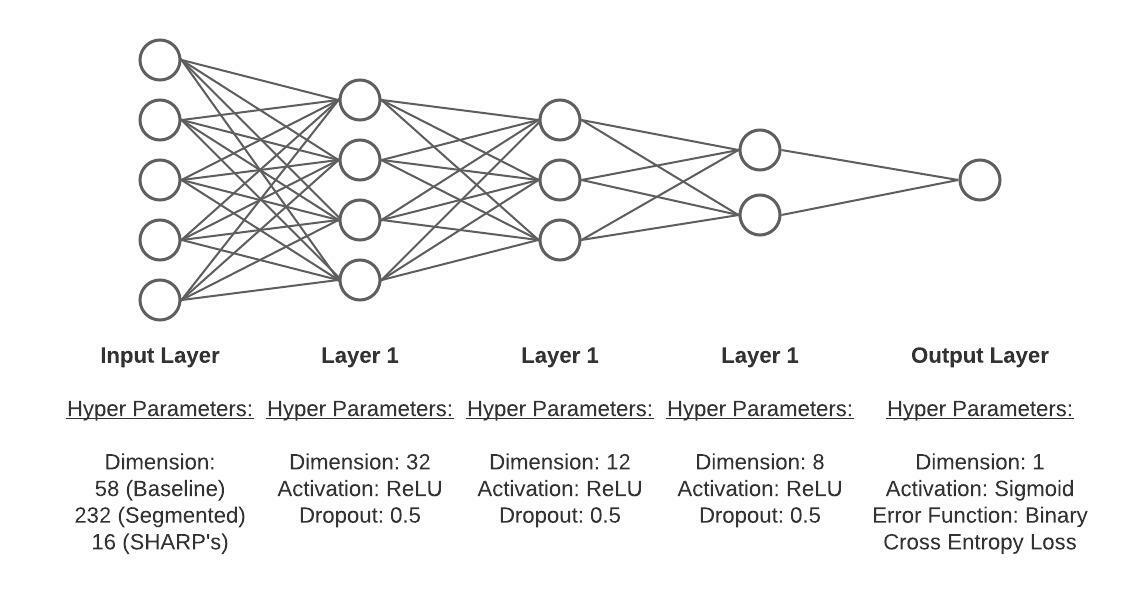
\includegraphics[width=\linewidth]{ThesisFilePkg/figures/methods/ann.jpeg}
    \caption{The Artificial Neural Network Design}
    \label{fig:ann}
\end{figure}

Figure \ref{fig:ann} indicates that the input dimension was fixed, but I also changed the dimension to the top 10 elements as well for each feature set.

Due to the heavily unbalanced feature set, in my training data, I weighted flaring data points as 100 and non flaring data points as 10 in my binary cross entropy loss function. I also decreased the weights of ARs near the 24 hour mark. Each AR data point is assigned a value of $t$. For flaring ARs, this is simply the time until the next M+ flare. For non flaring regions, $t$ is treated as infinite and the weight is taken as $t \rightarrow \infty$. I assign an asymptotic flaring weight ($a_f = 10$) and an asymptotic non flaring weight ($a_{nf} = 100$) that each describe the extremes of flaring and non flaring regions to my model (ie $t = 0$ and $t \rightarrow \infty$). I have a minimum weight ($w_min = 0.1$) equal to the weight of an AR that would occur in exactly 24 hours and two scaling terms: $a = 1$, $b = 30$ that scale the curvature of the climb of both flaring and non flaring weights, respectively. Overall, each AR weight is assigned:  

\[weight(t) = 
\begin{cases}
    (a_f - w_{min})(1 - e^{-\frac{(t - 24)^2}{24a}}) + w_{min} \quad t \in (0, 24]\\
    (a_{nf} - w_{min})(1 - e^{-\frac{(t - 24)^2}{24b}}) + w_{min} \quad t \in [24, \infty)
\end{cases}
\]

and the distribution of weights with respect to time till flare is shown in figure \ref{fig:weights}.
\begin{figure}
    \centering
    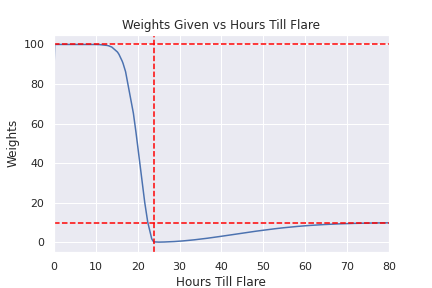
\includegraphics[width=0.5\linewidth]{ThesisFilePkg/figures/methods/weights.png}
    \caption{The weights assigned to each AR data point given it's time till flare in the Binary Cross Entropy Loss Function. Non flaring ARs are taken as $t \rightarrow \infty$. The left hand assymptote (top red line) is 100, the right hand asymptote (bottom red line) is 10 and the minimum weight (middle vertical red line) is 0.1.}
    \label{fig:weights}
\end{figure}

\subsection{Graph Models}

For my Graph feature set, I need to first represent each Graph as a vector (through a node embedding), then pass this vector into the same (optimized) models described above. This simplifies the process of comparing the performance of the Graph feature set by using the same models with that added step of node embedding. I tried two methods of node embeddings: a Graph neural network autoencoder and node2vec. I found that node2vec had too many parameters to tune (in addition to the massive amounts of parameters to tune in the feature extraction algorithm itself), which made it unwieldy for the hundreds of thousands of data points I had access to. Therefore, I used a Graph neural network for my primary results. 

An autoencoder is designed to take in an input, and transform it in some way to a (usually lower-dimensional. In this case, it transforms a Graph into a low dimensional fixed vector space) by an encoder layer then decodes the vector into the input data format with a minimal amount of error between the initial input and decoded output. 

Let the original Graph $G$ be a collection of nodes $v$ (a 58-dimensional vector representing all the physical features of that node) and edges $e$ (that connect two nearby nodes).  The Graph neural network takes the neighbors of each node $v$ ($n(v)$) and  transforms them into a new space. After transformation, the new vector $v’$ becomes:

$$v'= \sigma (W*v + \sum_{n(v)} W*n(v))$$ 

Where $\sigma$ is some activation function (I used ReLU), and $W$ is a  learn-able weight matrix. This transformation is done for each node in the Graph, and the same transformation is applied to the neighbors of $v$. This process can be repeated multiple times (indicating the number of Graph layers). I chose only one layer. 

The final Graph $G'$ is a transformed version of the original Graph $G$ with the same topology, only the original vectors $v$ are represented as transformed vectors $v'$. Then, I take the average of all nodes as the final vector encoding. This vector is supposed to represent all aspects of the Graph including the Graph topology and vector values of each node. The decoder takes in this vector and predicts a theoretical new Graph ($\hat{G}$) including both topology and node values that is ideally exactly the same as Graph $G$. The error between the two Graphs represents the machine learning loss function and is taken as the Graph edit distance plus the difference in average nodes:

$$d(G, \hat{G}) = GED(G, \hat{G}) + |\frac{1}{N}\sum_{v \in G}v - \frac{1}{\hat{N}}\sum_{\hat{v} \in \hat{G}}\hat{v}|$$

The final vector could then be used in all the previously mentioned models, however, I chose to only test this vector embedding on the Artificial Neural Network. This is because, although the idea of Graph encoding could work for detailed Graphs representing each AR, a majority of Graphs in my feature set were seemingly invalid. Many Graphs had no nodes at all (a small amount of which surprisingly flared in 24 hours), and many Graphs were composed of disjoint Graphs. This means that the Graph embedding step would label all no-node Graphs the same (flaring or not), and would struggle to find any sort of relationship between nodes that weren't connected to one another (because there would be no update step in the primary Graph neural network step that encodes the Graph into a vector). 

I will share my results for this model in the findings chapter, but they should not be taken significantly because of the previously mentioned issues.


\subsection{Other Models}

The above models were compared between Full and Segmented (with the exact algorithm explained below). I was also interested in changing the problem space to find the most optimal model. I tried various other models including ones that implemented time series analysis into the data. Using the same model proposed above, I created a \textbf{time stacked} neural network, where I took the 10 most important features, and stacked vectors with a distance of $s$ hours from one another and overall lookback of $l$ (meaning a total hour look back of $s \times l$). Data were considered $batch \times lookback \times 10$ dimensional input vectors and passed to the neural network as is. 

I also designed an LSTM binary classifier, Artificial Neural Network Regression model, LSTM Auto Encoder and Artificial Neural Network Auto Encoder, but I will not be considering the results of these models for the scope of this study.
